\documentclass[11pt]{article}

\usepackage[margin=1in]{geometry}
\usepackage[T1]{fontenc}
\usepackage[utf8]{inputenc}
\usepackage{amsmath,amssymb}
\usepackage{booktabs}
\usepackage{graphicx}
\usepackage{float}
\usepackage{hyperref}
\usepackage{xcolor}
\usepackage{enumitem}
\usepackage{array}

\hypersetup{
  colorlinks=true,
  linkcolor=blue,
  urlcolor=blue,
  citecolor=blue
}

\title{Final Report: MLSE Project\\Event-Type Player Similarity in the PlayerBERT Pipeline}
\author{Ziheng Lin}
\date{\today}

\begin{document}

\maketitle

\section{1. Intro}

This report investigates the following question: \emph{for a given player, who is most similar under a specific event type, such as \texttt{Pass} or \texttt{Carry}?} The question arises from a limitation of global player similarity, in which a single embedding per player conflates many distinct behaviors and therefore obscures action-specific structure. To address this issue, I develop an end-to-end pipeline built on StatsBomb open data and 360 context, including data preprocessing, event-level representation learning, sequence-level modeling, and a downstream retrieval stage; the primary emphasis of the report is the Event-Type Player Similarity component because it provides the most direct answer to the research question.

\section{2. Data \& Data Processing}

\subsection{Data used}

The project uses StatsBomb open data and relies on three aligned sources from the repository:
\begin{itemize}[leftmargin=*]
  \item event JSON files from \texttt{open-data/data/events},
  \item 360 freeze-frame JSON files from \texttt{open-data/data/three-sixty},
  \item lineup JSON files from \texttt{open-data/data/lineups}.
\end{itemize}

These sources are merged to produce the processed file \texttt{events360\_v4.jsonl}, which serves as the principal input for EventEncoder training, PlayerBERT training, and the downstream event-type similarity cache.

\begin{table}[H]
\centering
\caption{Data sources used in the pipeline.}
\label{tab:data-sources}
\begin{tabular}{>{\raggedright\arraybackslash}p{0.28\textwidth} >{\raggedright\arraybackslash}p{0.62\textwidth}}
\toprule
Source & Role in the pipeline \\
\midrule
StatsBomb event files & Core event metadata such as type, player, team, timestamp, pass fields, shot fields, and raw locations. \\
StatsBomb 360 frames & Local spatial context around the event through \texttt{freeze\_frame} and visible area. \\
Lineup files & Positional metadata used to replace \texttt{pass.recipient} with \texttt{recipient\_position}. \\
\bottomrule
\end{tabular}
\end{table}

\subsection{Processing steps}

The preprocessing logic is implemented in \texttt{scripts/preprocess\_360\_events.py}. The pipeline proceeds in the following stages:
\begin{enumerate}[leftmargin=*]
  \item Match each 360 frame to its event using the shared event identifier, \texttt{event\_uuid}.
  \item Copy event attributes and append 360 context, especially \texttt{freeze\_frame} and \texttt{visible\_area}.
  \item Load lineup data and replace \texttt{pass.recipient} with \texttt{pass.recipient\_position} so that tactical role is preserved while direct recipient identity is removed.
  \item Normalize boolean fields so missing values become \texttt{False}.
  \item Normalize categorical fields so missing values become \texttt{Unknown}.
  \item Bucketize continuous variables into coarse categories, including top-level location, pass end location, pass length, pass angle, shot end location, and shot xG.
  \item Keep actor location and freeze-frame lists because they are consumed directly by the EventEncoder.
  \item Write the final enriched dataset as one JSON object per line to \texttt{events360\_v4.jsonl}.
\end{enumerate}

These design choices are intended to improve both statistical stability and representational consistency. Bucketization reduces the cardinality of tabular features, normalization ensures that missingness is encoded consistently across events, and the use of recipient position instead of recipient identity helps retain tactical information while reducing direct player-identity leakage.

\section{3. Methods}

\subsection{Overview}

The full pipeline contains three connected modeling components: an EventEncoder, a sequence-level PlayerBERT model, and an event-type-conditioned retrieval layer. Their respective roles are summarized in Table~\ref{tab:methods-overview}.

\begin{table}[H]
\centering
\caption{Methods used in the project and their motivation.}
\label{tab:methods-overview}
\begin{tabular}{>{\raggedright\arraybackslash}p{0.24\textwidth} >{\raggedright\arraybackslash}p{0.66\textwidth}}
\toprule
Model / component & Motivation and utility \\
\midrule
EventEncoder & Learn a contextualized embedding for a single event by combining event attributes with 360 spatial context. This is the core representation used throughout the project. \\
PlayerBERT & Model ordered per-player event sequences within matches so that temporal structure is captured, rather than treating events independently. \\
Event-Type Player Similarity & Reuse the pretrained EventEncoder to build player profiles conditioned on one event type, so the system can answer focused questions such as who passes like a given player. \\
\bottomrule
\end{tabular}
\end{table}

\subsection{EventEncoder}

The EventEncoder is trained using masked attribute modeling and combines three complementary components:
\begin{itemize}[leftmargin=*]
  \item a Transformer encoder over discrete event features,
  \item an MLP-based set encoder over 360 freeze-frame players,
  \item a gated fusion layer that merges event information and frame information.
\end{itemize}

The event branch captures \emph{what} happened through structured event attributes, while the frame branch captures \emph{where} the action took place relative to surrounding players. A gating mechanism fuses these two views into a single event representation in $\mathbb{R}^{128}$.

\subsection{PlayerBERT}

PlayerBERT operates at the sequence level. It groups events by player and match, orders them by timestamp, and applies masked event modeling over event embeddings. In the current pipeline, the EventEncoder is kept frozen and used as the embedding initializer. This stage is intended to capture within-match temporal structure and thereby support more global player representations than event-level modeling alone.

\subsection{Event-Type Player Similarity}

The main method studied in this report is Event-Type Player Similarity. For each event with player ID $p$ and event type $t$, the pretrained EventEncoder produces an embedding $\mathbf{e}_i$. These embeddings are then aggregated by player and event type to form a profile vector:
\[
\mathbf{v}_{p,t} = \frac{\sum_i \mathbf{e}_i}{n_{p,t}},
\]
where $n_{p,t}$ is the number of stored events for player $p$ under event type $t$.

This formulation is useful because it addresses behavior-specific questions rather than broad whole-player comparisons. It is also computationally efficient, since the implementation stores only one running sum and one count for each distinct $(p,t)$ pair instead of materializing every event embedding.

At query time, the system compares a query profile against all valid candidate profiles for the same event type using cosine similarity. Both the query player and the candidate player must satisfy a minimum support threshold, \texttt{min\_count}, so that retrieval is grounded in a sufficient number of observed events.

\section{4. Results}

\subsection{Built cache summary}

The current cache was constructed from \texttt{events360\_v4.jsonl} using the pretrained EventEncoder checkpoint. Table~\ref{tab:summary} summarizes the resulting artifact.

\begin{table}[H]
\centering
\caption{Summary statistics of the built event-type profile cache.}
\label{tab:summary}
\begin{tabular}{lr}
\toprule
Metric & Value \\
\midrule
JSONL rows read & 1{,}027{,}908 \\
Events encoded & 1{,}027{,}857 \\
Skipped (no \texttt{player.id}) & 51 \\
Distinct players & 2{,}409 \\
Distinct event types & 22 \\
Stored $(p,t)$ profile cells & 31{,}039 \\
\bottomrule
\end{tabular}
\end{table}

These statistics indicate that the retrieval layer scales to more than one million event rows while still producing a compact cache of slightly more than thirty-one thousand player-event-type profiles.

\subsection{Event-type distribution}

Figure~\ref{fig:event-type-totals} shows the total count of events per event type in the profile cache.

\begin{figure}[H]
\centering
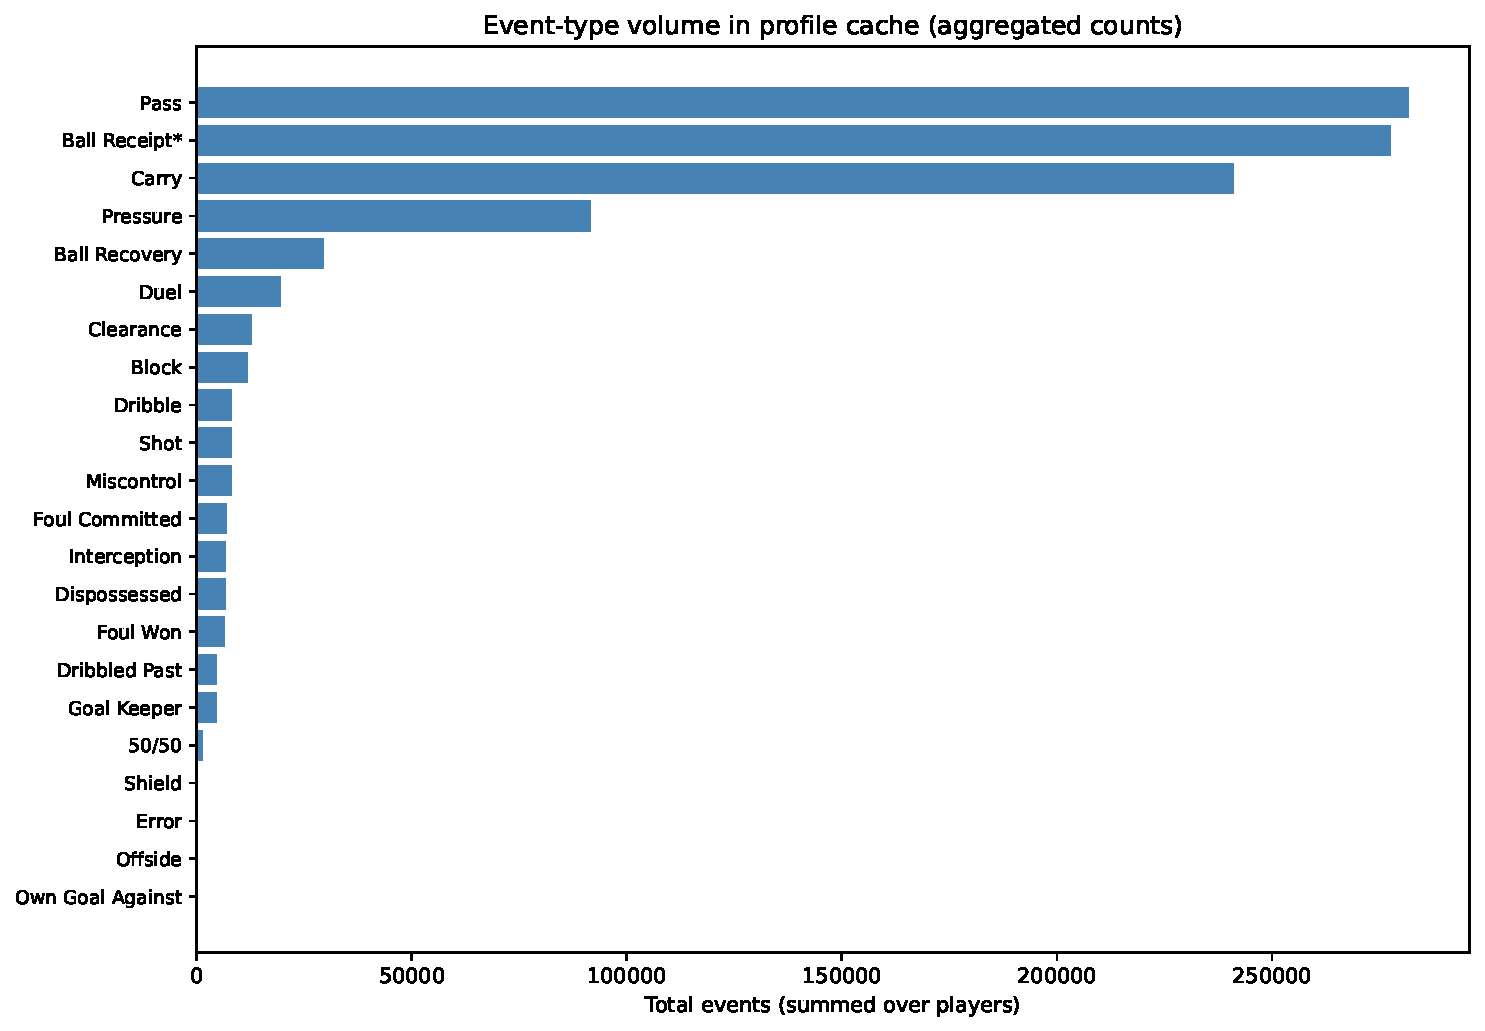
\includegraphics[width=0.82\textwidth]{../slides/figures/event_type_totals.pdf}
\caption{Total number of stored events by event type in the event-type profile cache. The distribution is head-heavy, with Pass, Ball Receipt*, and Carry dominating the cache.}
\label{fig:event-type-totals}
\end{figure}

This figure is directly relevant to the research question because event types with larger support, especially \texttt{Pass} and \texttt{Carry}, permit more stable event-type-conditioned comparisons across a large number of players.

\subsection{Support distribution across profiles}

Figure~\ref{fig:count-distribution} shows the support distribution over all stored $(p,t)$ profiles.

\begin{figure}[H]
\centering
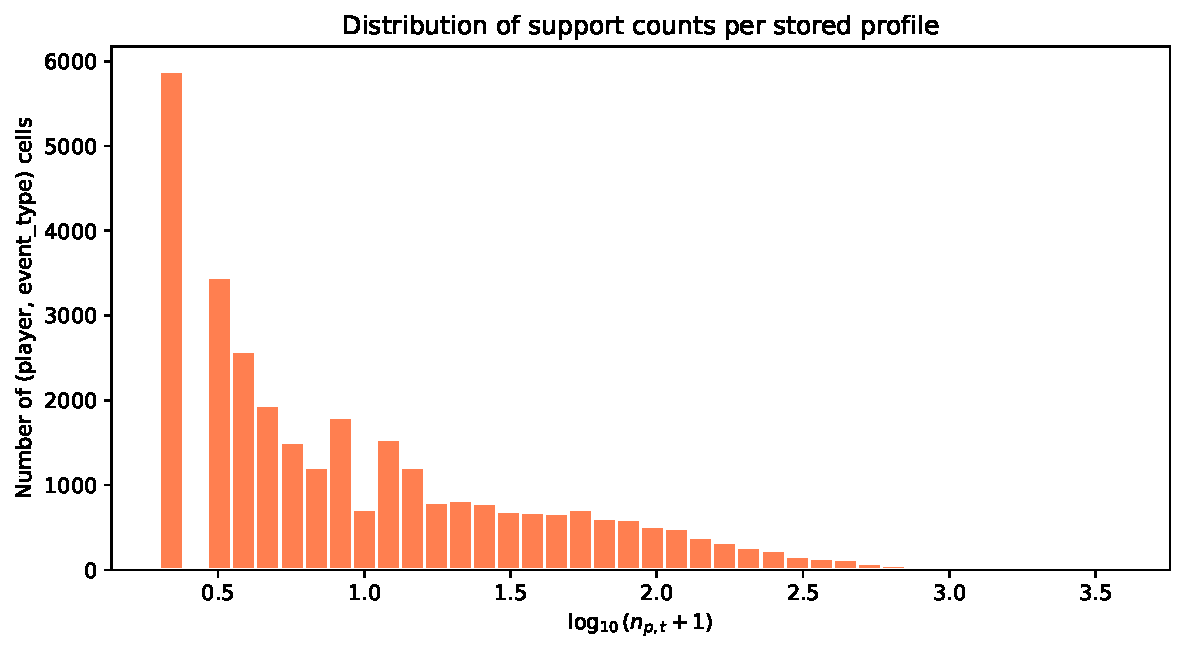
\includegraphics[width=0.75\textwidth]{../slides/figures/profile_count_distribution.pdf}
\caption{Distribution of support counts across stored player-event-type profiles, plotted on a log scale. This motivates the use of a minimum count threshold during querying.}
\label{fig:count-distribution}
\end{figure}

The figure shows that many player-event-type cells have moderate support, while a smaller subset has very high support. This pattern justifies the use of \texttt{min\_count} in order to avoid unstable retrieval for rare event types.

\subsection{Example retrieval result}

Table~\ref{tab:query-example} shows one \texttt{Pass} query example from the slides, using \texttt{top-k=5} and \texttt{min-count=20}.

\begin{table}[H]
\centering
\caption{Example nearest neighbors for a pass-profile query.}
\label{tab:query-example}
\begin{tabular}{>{\raggedright\arraybackslash}p{0.42\textwidth}rr}
\toprule
Player & Similarity & Count \\
\midrule
Alexandra Morgan Carrasco & 0.9850 & 75 \\
Borja Iglesias Quintas & 0.9844 & 74 \\
Harry Kane & 0.9913 & 21 \\
Aitana Bonmati Conca & 0.9899 & 37 \\
Alphonso Davies & 0.9899 & 22 \\
\bottomrule
\end{tabular}
\end{table}

This result is important for interpretation. The nearest neighbors can span leagues and genders because the model clusters \emph{how} a pass appears in context rather than \emph{who} the player is demographically. This is precisely why event-type-conditioned similarity is more informative than a single global embedding when the research question is action-specific.

\section{5. What comes next?}

Several extensions would strengthen the project further. First, profile aggregation could be made more expressive by replacing simple means with trimmed means or weighted means. Second, the same framework could be conditioned on finer facets such as \texttt{pass.height.name} or body part. Third, league-aware normalization could improve comparability across competitions. Finally, the event-type retrieval layer could be integrated more directly with PlayerBERT outputs so that action-level specificity and temporal structure are modeled jointly.

\appendix
\section{6. Appendix: technical aspects of the methods}

\subsection{Assumptions behind data processing}

The preprocessing pipeline relies on several assumptions:
\begin{itemize}[leftmargin=*]
  \item event IDs and 360 frame IDs are aligned correctly through \texttt{event\_uuid},
  \item replacing pass recipients with recipient positions preserves tactical meaning while reducing identity leakage,
  \item bucketizing continuous values is acceptable because coarse tactical categories are more important than exact raw values for this task,
  \item missing booleans and categoricals can be normalized safely into default tokens.
\end{itemize}

\subsection{Assumptions behind the models}

The EventEncoder assumes that a single event can be represented adequately through a combination of tabular event attributes and local 360 context. The frame encoder further assumes that mean-pooling over visible players is sufficient to summarize the local spatial neighborhood.

PlayerBERT assumes that ordered event sequences within a match contain meaningful temporal structure and that a Transformer encoder can learn this structure from event embeddings.

Event-Type Player Similarity assumes that averaging event embeddings within one event type is sufficient to produce a meaningful marginal profile for a player under that action category.

\subsection{Alignment between modeling and processed data}

The models depend directly on the processed data schema. EventEncoder training uses discrete feature IDs derived from flattened and normalized event fields, while the frame encoder consumes the actor location and the freeze-frame player list. Consequently, the \texttt{feature\_vocab} saved in \texttt{event\_encoder\_mam.pt} must match the exact processed feature space observed at inference time.

\subsection{Model and data limitations}

The principal limitations are:
\begin{itemize}[leftmargin=*]
  \item mean pooling may mix multiple sub-styles within the same event type,
  \item rare event types produce noisier retrieval even when they meet a low support threshold,
  \item the current retrieval method does not model temporal order directly,
  \item the quality of the learned representation depends on consistency between the preprocessing pipeline and the saved checkpoint.
\end{itemize}

Despite these limitations, the event-type retrieval layer remains a useful and interpretable downstream application of the learned event representations.

\end{document}
